\documentclass[12pt,a4]{article}
\usepackage[]{graphicx}\usepackage[]{xcolor}
% maxwidth is the original width if it is less than linewidth
% otherwise use linewidth (to make sure the graphics do not exceed the margin)
\makeatletter
\def\maxwidth{ %
  \ifdim\Gin@nat@width>\linewidth
    \linewidth
  \else
    \Gin@nat@width
  \fi
}
\makeatother

\definecolor{fgcolor}{rgb}{0.345, 0.345, 0.345}
\newcommand{\hlnum}[1]{\textcolor[rgb]{0.686,0.059,0.569}{#1}}%
\newcommand{\hlstr}[1]{\textcolor[rgb]{0.192,0.494,0.8}{#1}}%
\newcommand{\hlcom}[1]{\textcolor[rgb]{0.678,0.584,0.686}{\textit{#1}}}%
\newcommand{\hlopt}[1]{\textcolor[rgb]{0,0,0}{#1}}%
\newcommand{\hlstd}[1]{\textcolor[rgb]{0.345,0.345,0.345}{#1}}%
\newcommand{\hlkwa}[1]{\textcolor[rgb]{0.161,0.373,0.58}{\textbf{#1}}}%
\newcommand{\hlkwb}[1]{\textcolor[rgb]{0.69,0.353,0.396}{#1}}%
\newcommand{\hlkwc}[1]{\textcolor[rgb]{0.333,0.667,0.333}{#1}}%
\newcommand{\hlkwd}[1]{\textcolor[rgb]{0.737,0.353,0.396}{\textbf{#1}}}%
\let\hlipl\hlkwb

\usepackage{framed}
\makeatletter
\newenvironment{kframe}{%
 \def\at@end@of@kframe{}%
 \ifinner\ifhmode%
  \def\at@end@of@kframe{\end{minipage}}%
  \begin{minipage}{\columnwidth}%
 \fi\fi%
 \def\FrameCommand##1{\hskip\@totalleftmargin \hskip-\fboxsep
 \colorbox{shadecolor}{##1}\hskip-\fboxsep
     % There is no \\@totalrightmargin, so:
     \hskip-\linewidth \hskip-\@totalleftmargin \hskip\columnwidth}%
 \MakeFramed {\advance\hsize-\width
   \@totalleftmargin\z@ \linewidth\hsize
   \@setminipage}}%
 {\par\unskip\endMakeFramed%
 \at@end@of@kframe}
\makeatother

\definecolor{shadecolor}{rgb}{.97, .97, .97}
\definecolor{messagecolor}{rgb}{0, 0, 0}
\definecolor{warningcolor}{rgb}{1, 0, 1}
\definecolor{errorcolor}{rgb}{1, 0, 0}
\newenvironment{knitrout}{}{} % an empty environment to be redefined in TeX

\usepackage{alltt}
\newcommand{\SweaveOpts}[1]{}  % do not interfere with LaTeX
\newcommand{\SweaveInput}[1]{} % because they are not real TeX commands
\newcommand{\Sexpr}[1]{}       % will only be parsed by R



% ---- Metadata ---- %

\title{Honesty by Convenience: Corruption Tolerance in Ecuador}
\author{Daniel Hernán Sánchez Pazmiño}
\date{June 2022}

% ---- Load Packages ---- %

% Math

\usepackage{savesym} % Need to "save" the command that is already defined \varTheta

\usepackage{amsmath}
  \savesymbol{varTheta} 

% Fonts

% To set the TNR font for both text and equations:

\usepackage{mathspec}
  \setallmainfonts(Digits,Greek,Latin){Times New Roman}
\restoresymbol{MTP}{varTheta}

% Formatting

\usepackage{setspace}
  \doublespacing

\usepackage[margin = 1in]{geometry}

% Citation & Bibliographies

\usepackage[backend = biber, style = apa, citestyle = apa]{biblatex}
  \addbibresource{refs.bib}
  
% For tables:

\usepackage{siunitx} % For the modelsummary tables
\usepackage{booktabs} % For the modelsummary tables
  \newcolumntype{d}{S[input-symbols = ()]}
\usepackage{caption}
\usepackage{multirow}
\usepackage[flushleft]{threeparttable}
  
% Other packages

\usepackage{csquotes} % For quotation marks

\usepackage{epigraph} % For epigraph
  \setlength\epigraphwidth{9cm}
  \setlength\epigraphrule{1pt}

\usepackage{float} % For the H float option- only used in emergencies (lol)

\usepackage{textcomp} % For the registered trademark symbol.

% Always load these packages at the end of the preamble:

\usepackage{hyperref}

% ---- R Stuff to be used in the whole document ----

% Here I will execute or source R code through chunks that I need to use throughout the whole document.

% General settings



% Load the data by sourcing the data manipulation script. Note that survey design objects are indeed created in this script.




\begin{document}
% Introduction .Rnw File


\section{Introduction}

\epigraph{\textit{Con guantes de operar hago un pequeño bolo de lodo suburbano. Lo hecho a rodar por esas calles: los que se tapen las narices le habrán encontrado carne de su carne}.}{Pablo Palacio, \textit{Un hombre muerto a puntapiés}.} \nocite{Palacio.2018}
\vspace{-0.8cm}
\epigraph{\textit{[...] por la certeza de que reconocer nuestros errores es el único camino para reconocer nuestros valores.}}{Jorge Enrique Adoum, \textit{Ecuador: señas particulares}..}

\enquote{Even if you are from [my political party], I will fulfill my duties. If you steal, steal well!  Justify well! But do not let your affairs be seen, comrades\footnote{Translated from Cerda, 2021 in \cite[para. 2]{PlanV.2021}}}. Uttered publicly by Rosa Cerda, Ecuadorian congresswoman for the Napo province \parencite{Castro.2021}, these comments met widespread criticism around the country, although the remarks were initially met by cheers from an audience of the indigenous movements convention she was addressing. This happened soon after a heated presidential election where corruption was one of the most important debate topics. Both candidates denounced each other's alleged dishonest acts, and promised their voters to punish corrupt behavior and foster a clean government. However, Cerda's declarations did not transcend an eight day suspension \parencite{Ordonez.2021} and the whole event was soon almost completely forgotten by most citizens. 

This episode is only one of many corruption-related scandals that have happened in the last years in the country. It is almost as if these no longer outrage the average Ecuadorian: at most, they cause a sigh of disappointment or social media outrage which dwindles shortly after. A convicted former president as well as two vicepresidents impeached and removed on charges of corruption (\cite{Press.1222018}; \cite{Cabrera.2020}), along with other several major corruption scandals (\cite{BHCompliance.2021}; \cite{Espana.2020}) are some events which have contributed to Ecuador placing well above the corruption median in the world according to both Transparency International's and the World Bank's corruption indexes. 

% Perform all survey-robust tabulations by sourcing the R Script


Close to 90\% of voting-age Ecuadorians believe that at least half of politicians are corrupt and more than a quarter of them admit having been asked to pay or actually paid a bribe in 2019, according to the AmericasBarometer (AB) survey data. However, a mere 8.08\% consider that corruption is the most serious problem faced by the country and in fact 25.38\% of Ecuadorians believe that paying a bribe is justified, \enquote{given the way things are} \parencite[p. 96]{Moscoso.2018}. In fact, the data from the AB has shown that tolerance to corruption has risen 11.79 percentage points from 2014 to 2019. Furthermore, Figure \ref{fig:ctolmap} shows that Ecuador is also one of the countries with the highest corruption tolerance in the region.

% Corruption Tolerance Choropleth Map based on 2019 values

% Sorry, this map was done with the paid AmericasBarometer databases, so I cannot actually put my source code and have it executed by KNITR. USFQ students are free to access another version of the document, they must only email me. Third parties must wait until I do it with the free databases. The last appendix on this document shares the source code to compile the graph, but it won't work without the databse. Sorry!

\begin{figure}[htbp]
  \fbox{
    \begin{minipage}{\textwidth}
      \caption{Corruption Tolerance (\%) Choropleth Map in 2019}
      \label{fig:ctolmap}
      \begin{center}
      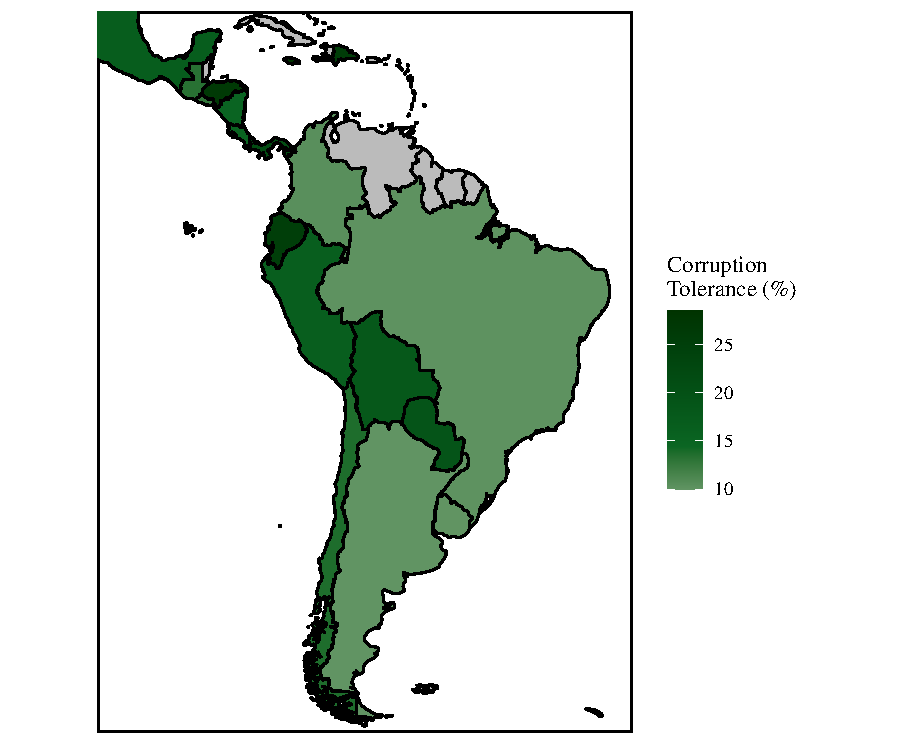
\includegraphics{images/ctol_map.pdf}
      \end{center}
      \textbf{Note:}
      A choropleth map showing corruption tolerance percentages across Latin America in 2019, where Ecuador places third in        the most corruption tolerant countries. Darker areas imply higher percentages of corruption tolerance. Figure                prepared by the author with data from the \textregistered AmericasBarometer 2018/19. 
    \end{minipage}
  }
\end{figure}

Corruption, if framed as any kind of inappropriate use of common power to benefit a select few at the expense of others \parencite{Warren.2004}, affects Ecuadorians extensively in their daily lives. According to \textcite{AlarconSalvador.2020}, up to 1.5 billion USD may be have been lost in 2019 due to corrupt practices in public contracting. During the decade-long Revolución Ciudadana regime, the local Anti-Corruption Comission estimates a 35 billion USD cost of corruption \parencite{RoaChejin.2020}. Ecuador has also seen increased COVID-19 vaccine inequality as top public officers inoculated non-priority subjects in their private circles \parencite{Taj.2021}, weakened public health services (\cite{Celi.2020}; \cite{Comercio.2021}; \cite{RoaChejin.2020}), policymakers charging fees for political positions (\cite{Espinosa.2021}; \cite{Gonzalez.2021}), lost Social Security funds \parencite{Pesantes.9152020}, among others. With the impairment of so many public services which Ecuadorians pay for and depend on, it would be expected that corrupt activities become publicly denounced and repudiated.

% Corruption Tolerance Time Series Graph

\begin{figure}[htbp]
\centering
\fbox{
\begin{minipage}{\textwidth}
\caption{Percent of Ecuadorians who justify corruption, by year}
\label{fig:ctoly}
\begin{knitrout}
\definecolor{shadecolor}{rgb}{0.969, 0.969, 0.969}\color{fgcolor}

{\centering 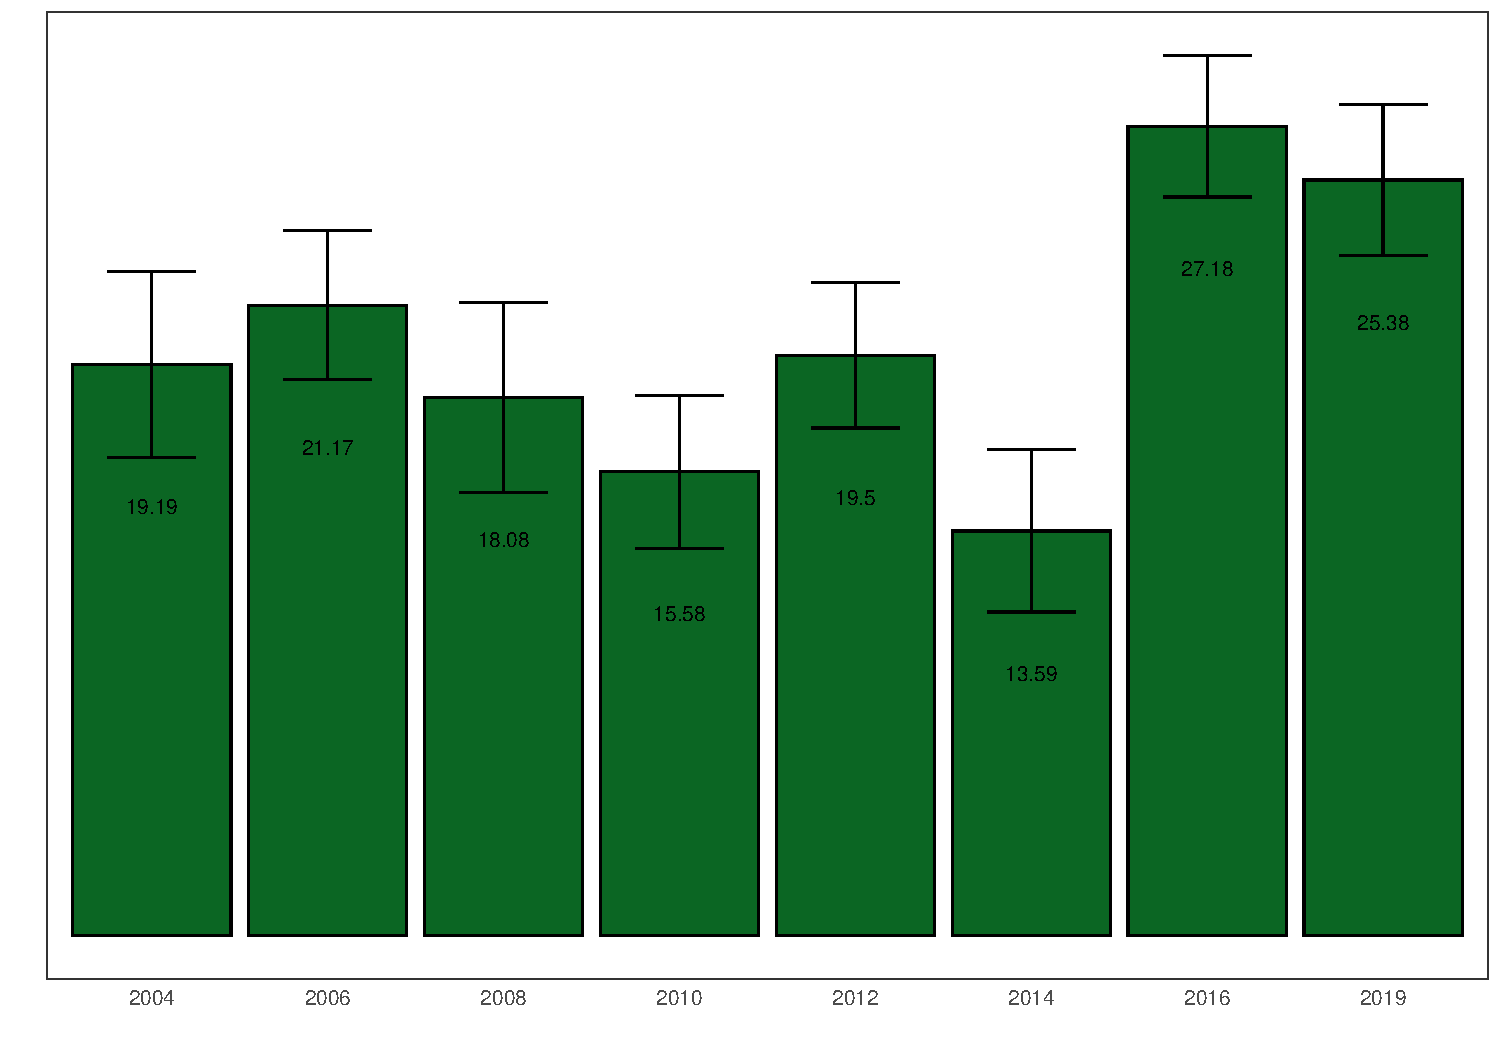
\includegraphics[width=\maxwidth]{figure/ctol_graph-1} 

}


\end{knitrout}
\textbf{Note:} The evolution of corruption tolerance for Ecuador. The largest increase is seen from 2014 to 2016. Error bars show 95\% confidence intervals, considering survey design effects. Figure prepared by the author, with the open-access AB data.
\end{minipage}}
\end{figure}

The largest increase in corruption tolerance was seen from 2014 to 2016, as it can be seen in Figure \ref{fig:ctoly}, where it increased from a historical low of 13.59 to a high of 27.18\%. This period coincides with two key events in the country. First, the popularity of a left-leaning and apparently omnipotent regime sharply dropped among accusations of corruption and poor management of the economy \parencite{Quillupangui.2016}. Second, a considerable economic recession hit the country which was mostly attributable to a commodity price collapse \parencite{Weisbrot.2017}. 

This study aims to explain the jump in corruption tolerance using survey data from the America's Barometer. The empirical analysis provides evidence that changes to the public's support of the political regime as well as a deteriorating economic environment came into play to increase corruption tolerance. The individual-level and across-time approach is a novelty in corruption literature and could be a better empirical approach to these kinds of research questions, as omitted-variable biases can be better controlled compared to cross-country approaches \parencite{Bergh.2017}. 

The mentioned events may have interacted with each other to cause political and economic turmoil as presidential elections approached in 2017 and many questioned the regime for the first time. Apart from the deterioration of the economy, the rule of President Rafael Correa saw its approval rating drop -15 percentage points according to the AB. These are significant changes in public opinion, so it is sensible to look at these as potential drivers for the increase in corruption tolerance. It should also be noted that historically, Ecuadorian citizens have tended to recognize corruption as an inevitable consequence of any political process, seemingly imagining a trade-off between corruption and public goods \parencite{Adoum.2000}. This account was confirmed by another public opinion in 2018, which estimates that 44\% of Ecuadorians justify corruption if it is done in exchange of goods and services provided by the public sector \parencite{Loaiza.2019}. Additionally, \textcite{Hurtado.2007} and \textcite{Adoum.2000} recognize multiple behavioral patterns in Ecuadorian citizens which lead to attitudes of resignation to the mechanisms of corruption, which may normalize corruption and thus create environments that foster its growth. 

Changes to the attitudes toward corruption can be as important to understand as the consequences or causes of actual corruption. First, a higher degree of corruption tolerance will eventually lead to larger corruption environments \parencite{Campbell.2014}. Social sanctions or rewards can significantly affect outcomes according to \textcite{Akerlof.1980}, even if these lead to smaller economic payoffs. Higher tolerance to corrupt acts, such as bribing, will mean that the social sanction of engaging in them is smaller, hence making the total payoff of the corrupt action higher, since a positive economic payoff to the corrupt individual is implied \parencite{Shleifer.1993}. However, corruption almost always entails that the economic payoff to the corrupt individual is done at the expense of the majority \parencite{Warren.2004}, thus affecting outcomes across all society, notably economic development and political stability \parencite{Singer.2016}. It thus becomes of prime importance to learn what drives corruption tolerance to be able to foster better policy-making and citizen attitudes which drive citizens away from enacting in and justifying corrupt actions.



\end{document}
